\subsection{Setup}
\label{subsec:netshaper-evaluation-setup}

\begin{figure}[!htb]
    \centering

    \begin{subfigure}{\columnwidth}
        \centering
        
\includegraphics[width=\columnwidth]{figures/netshaper/testbed-setup.png}
        \caption{Evaluation Setup with NetShaper}
        \label{fig:testbed-setup-with-netshaper}
    \end{subfigure}

    \begin{subfigure}{\columnwidth}
        \centering
        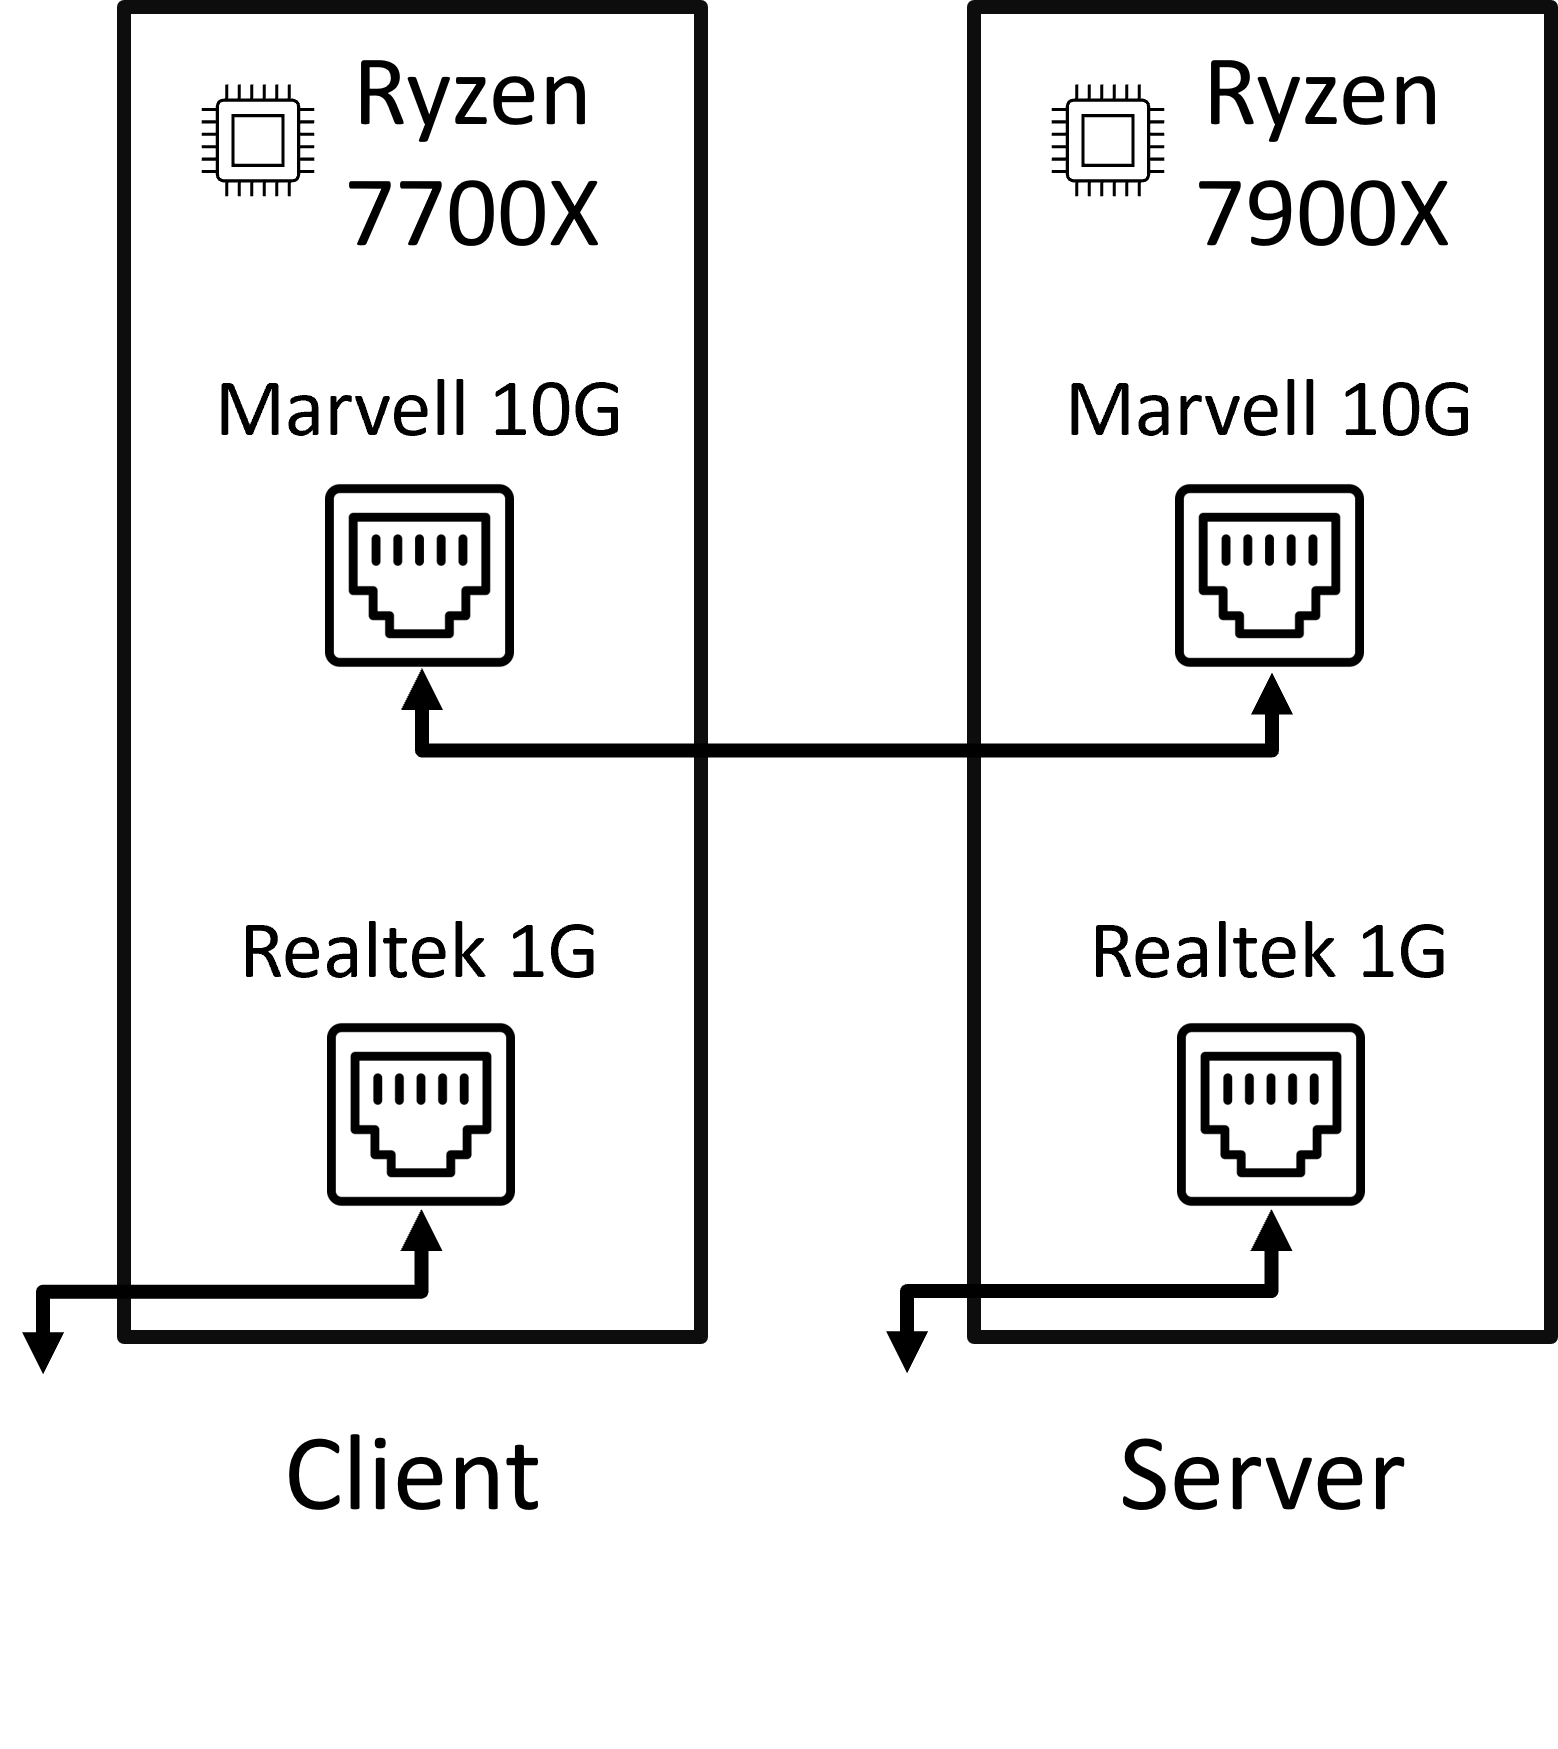
\includegraphics[width=0.5\columnwidth]{figures/netshaper/testbed-setup-no-middlebox.png}
        \caption{Evaluation Setup without NetShaper}
        \label{fig:testbed-setup-without-netshaper}
    \end{subfigure}

    \label{fig:testbed-setup}
    \caption{NetShaper setup}
\end{figure}

Our setup consists of four desktops, each of which consists of 32GB RAM, 1TB storage, one Marvell AQC113CS-B1-C 10G NIC, and one Realtek RTL8111 1G NIC.
We use the Realtek NIC only as a management NIC and do not run any experiments on it.
Three of the desktops have an AMD Ryzen 7 7700X processor with 8 physical cores.
One has a more powerful AMD Ryzen 9 7900X processor with 12 physical cores, which we use as the server.
We fix all cores on all desktops to run at 4.0 GHz to ensure that our results do not vary due to the varying CPU frequency.
The middleboxes are connected to each out via an additional Intel X550-T2 10G NIC.
The client and the server are connected to their local middleboxes via the Marvell 10G NIC.
This forms a linear topology, as outlined in \Cref{fig:testbed-setup}
All the desktops run Ubuntu 22.04.02 (Linux kernel version 5.19)

In all of the experiments, we do not place any restrictions on the client or the server applications.
All of the experiments contain a baseline setup wherein the client is directly connected to the server via the Marvell 10G NIC, bypassing the middleboxes.
For experiments i and ii, we use \textit{iperf3} \cite{iPerf3} as the client and server application.
For the rest of the experiments, we use \textit{Nginx} \cite{nginx} as the server and a modified 
\footnote{The wrk2 is modified to send asynchronous HTTP requests, and also report individual latencies for each request.}
wrk2 \cite{wrk2} as the client.